\section{Classification}\label{sec:classification}
\begin{center}
    \makebox[\columnwidth]{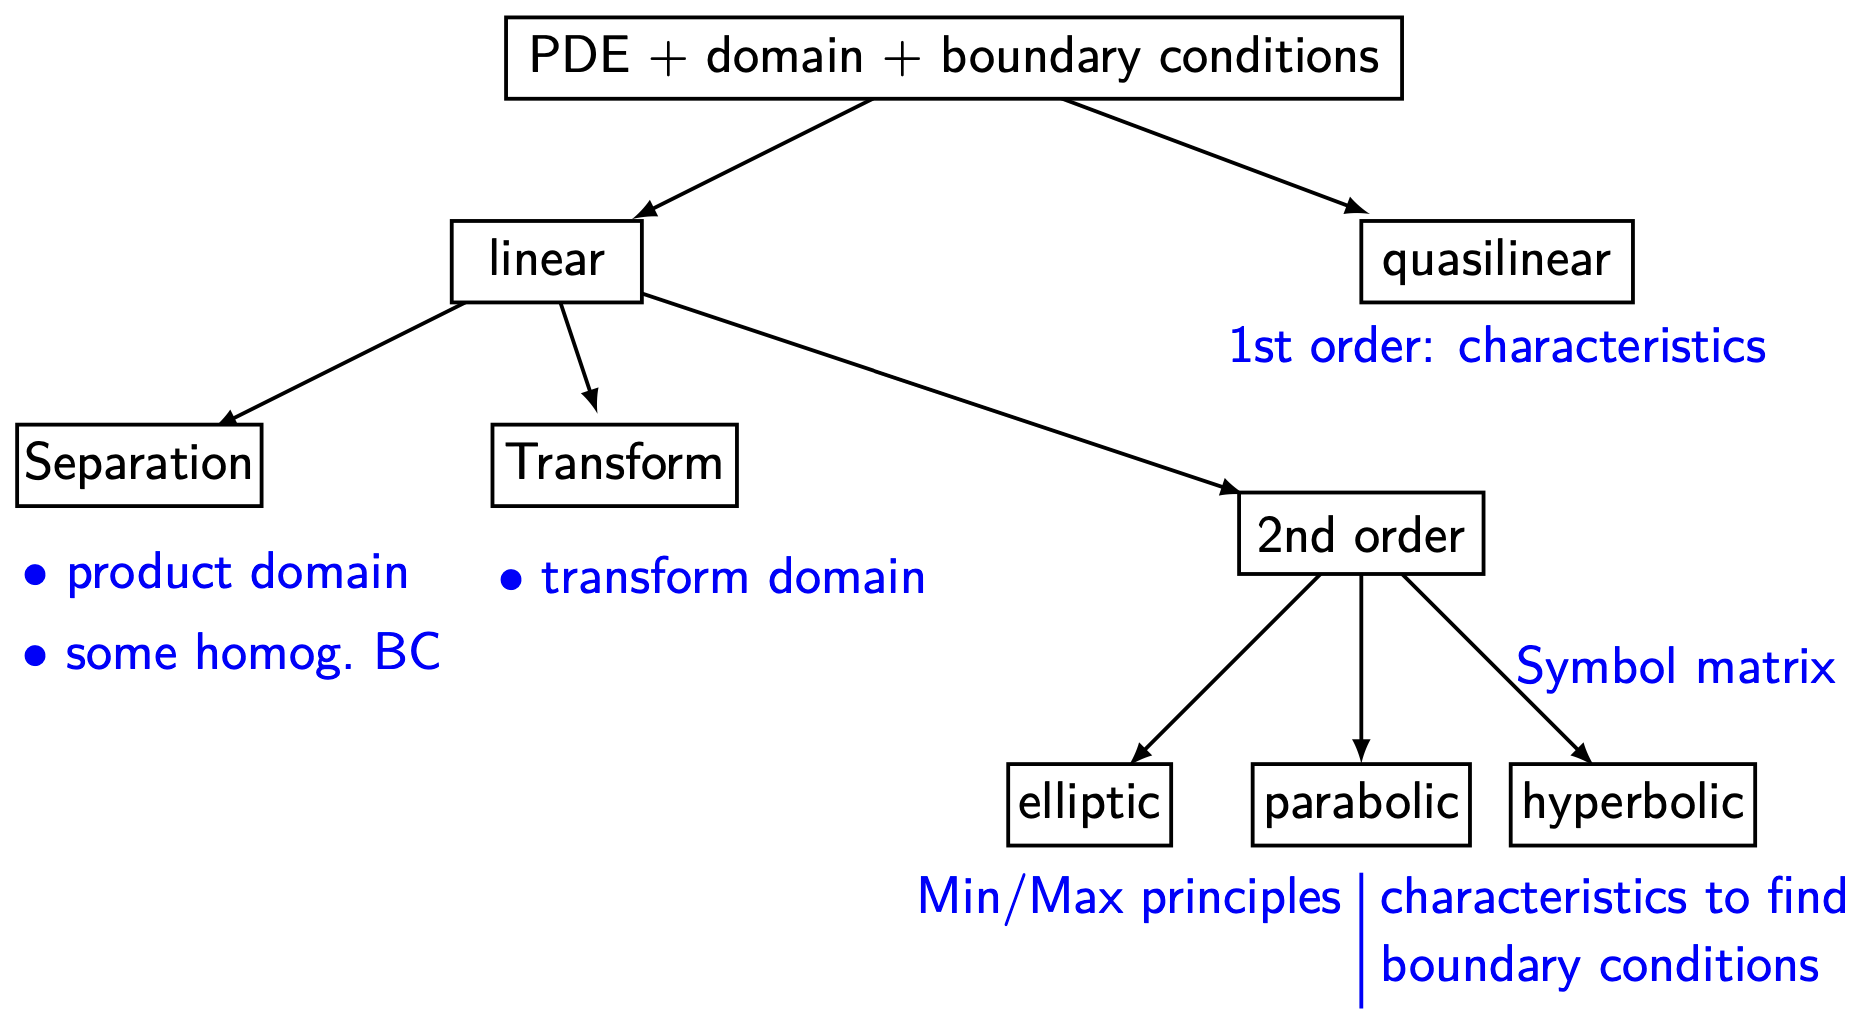
\includegraphics[width=0.9\columnwidth]{images/decision-tree}}
\end{center}

\subsection{Linearity}\label{subsec:linearity}
Given an equation involving a function $u(x), x\in\mathbb{R}$ and its derivatives,
there is a function $F$ describing the relation:
\begin{align*}
    F\left(
    \begin{matrix}
        x,y,z,p,q,s,t,r,\ldots                         \\
        \downarrow \text{(corresponding to)}\downarrow \\
        x, y, u, \frac{\partial u}{\partial x}, \frac{\partial u}{\partial y}, \frac{\partial^2 u}{\partial x^2},
        \frac{\partial^2 u}{\partial x\partial y},\frac{\partial^2 u}{\partial y^2}, \ldots
    \end{matrix}
    \right) = 0
\end{align*}
(common variable names $p_i\rightarrow\frac{\partial u}{\partial x_i}$ and
$t_{ij} \rightarrow\frac{\partial^2 u}{\partial x_i\partial x_j}$)

A PDE is \emph{linear} when function $F$ is linear in $u,p_1,\ldots,p_n,t_{11},\ldots,t_{nn},\ldots.$

A PDF is \emph{quasilinear} when function $F$ is linear in $p_1,\ldots,p_n,t_{11},\ldots,t_{nn},\ldots.$

For example, given the heat equation $u_t=\kappa u_{xx}$, $F$ would be $F(p_1,t_{22})=p_1-\kappa t_{22}$.

\subsection{2\textsuperscript{nd} Order PDEs: Symbol Matrix}

The symbol matrix of the 2\textsuperscript{nd} order partial differential operator

\begin{align*}
    L=\sum_{i,j=1}^{n}a_{ij}(x)\frac{\partial^2}{\partial x_i \partial x_j}+\sum_{i=1}^n b_i(x)\frac{\partial}{\partial x_i}+c(x)
\end{align*}

is the symmetric matrix

\begin{align*}
    A=
    \begin{bmatrix}
        a_{11} & a_{12} & \ldots & a_{1n} \\
        a_{21} & a_{22} & \ldots & a_{2n} \\
        \vdots & \vdots & \ddots & \vdots \\
        a_{n1} & a_{n2} & \ldots & a_{nn}
    \end{bmatrix}
\end{align*}

For example:

\begin{center}
    \makebox[\columnwidth]{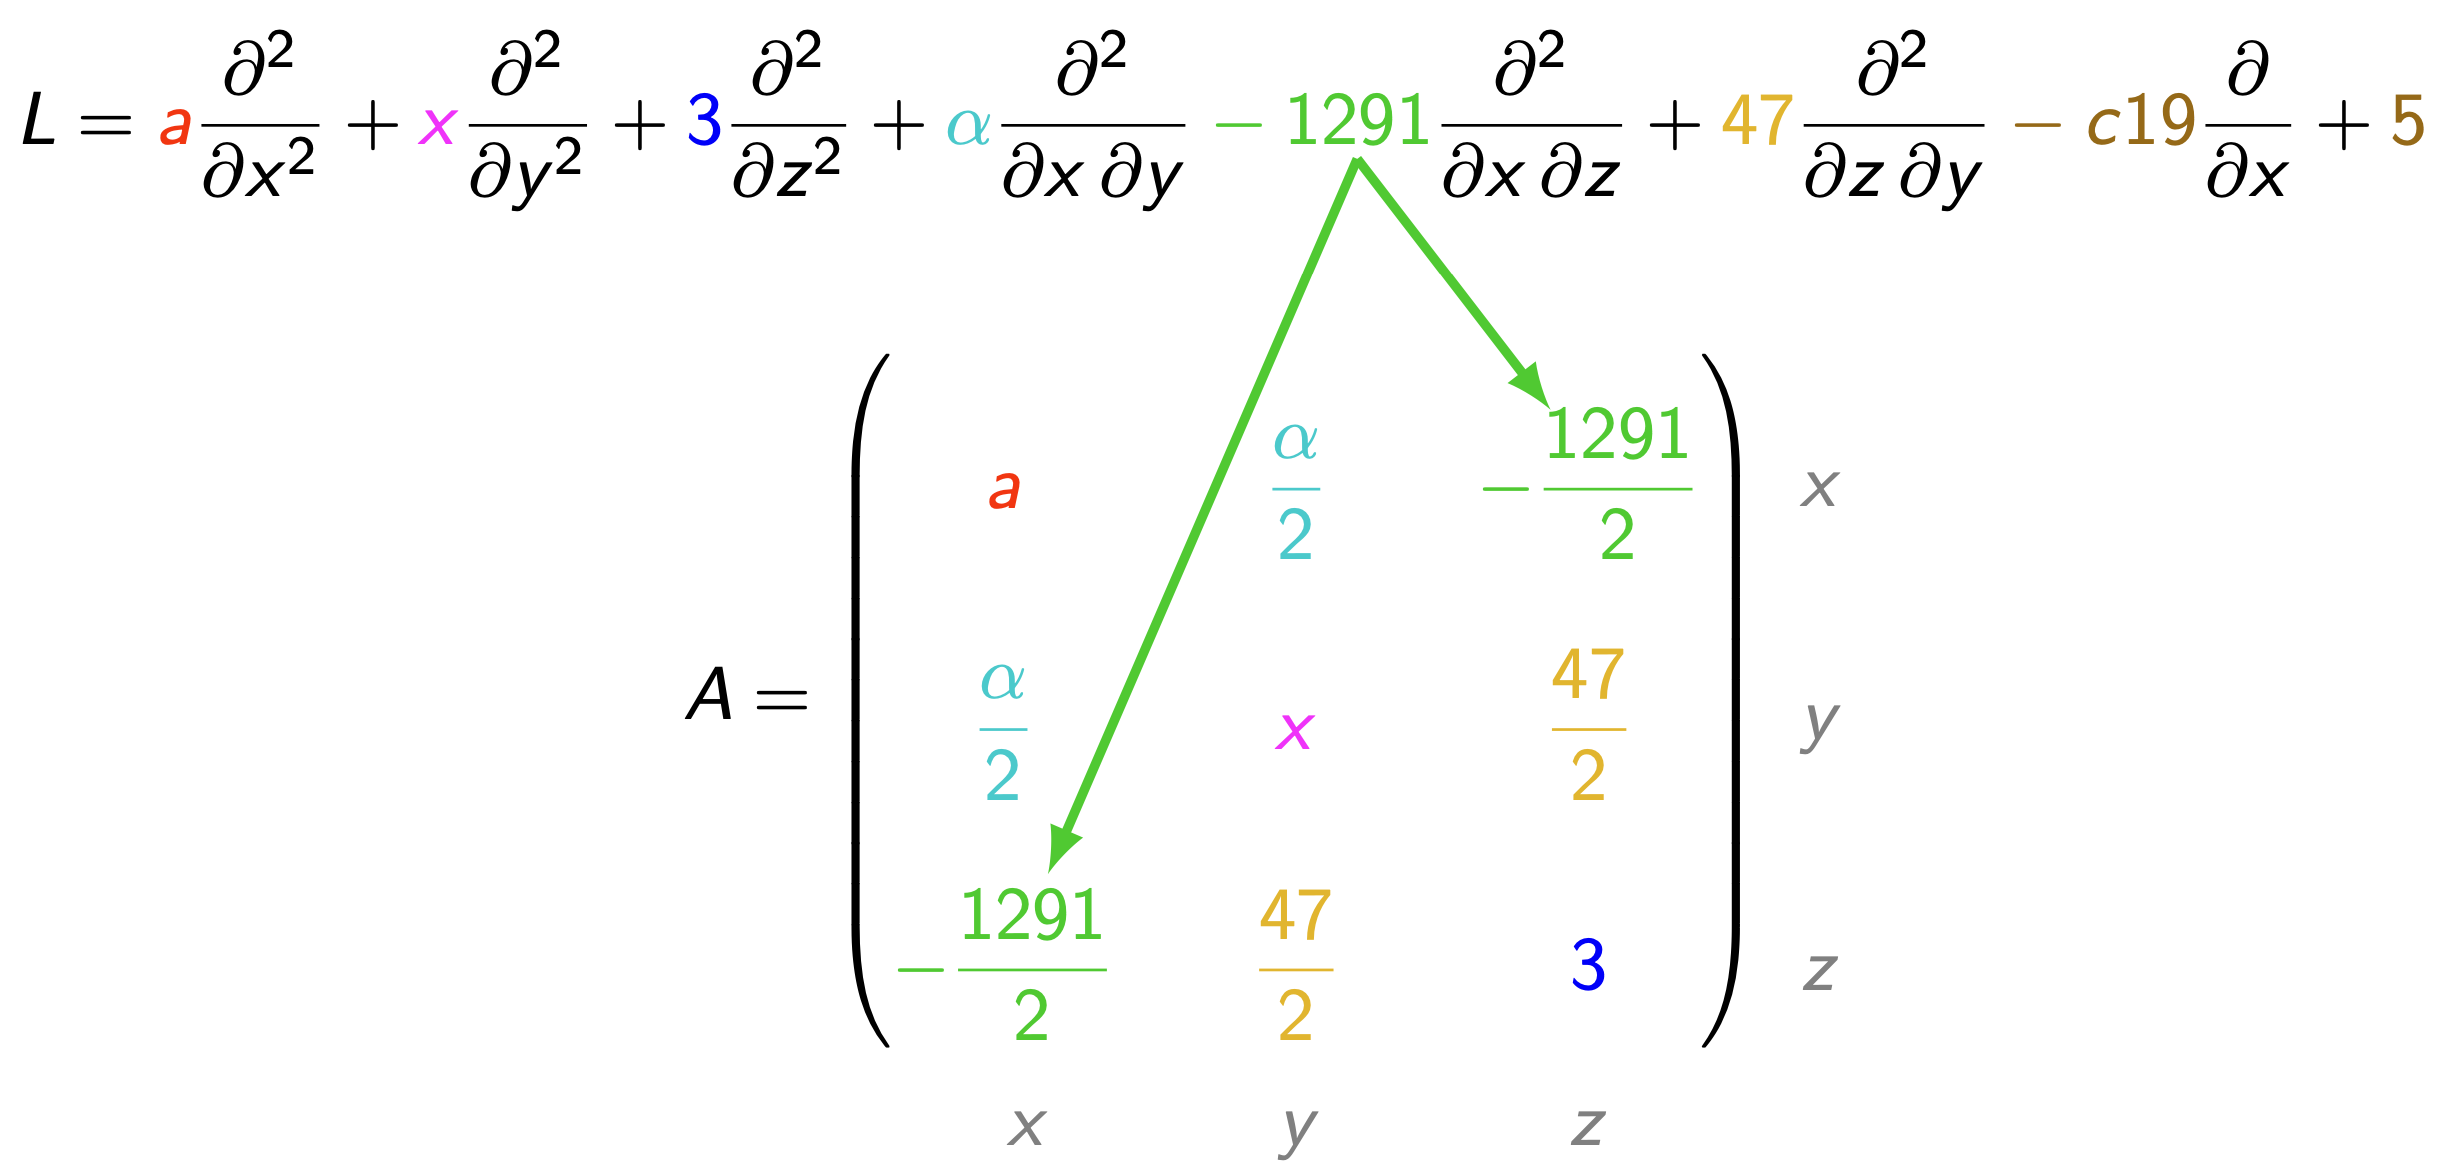
\includegraphics[width=0.9\columnwidth]{images/symbol-matrix}}
\end{center}

The type of equation can be inferred by the sign of the eigenvalues $\lambda_1,\ldots,\lambda_n$ of the symbol matrix.
Calculating the determinant ($\det A=\prod_i \lambda_i$) and trace ($\mathrm{tr}\ A=\sum_i \lambda_i$)
reveals information about the signs of its eigenvalues:

\subsubsection{Two Variables of PDE}

\begin{align*}
    \det A
    \left\{
    \begin{matrix}
        >0 & \text{elliptic (eigenvalues have same sign)}       \\
        =0 & \text{parabolic (at least one eigenvalue is zero)} \\
        <0 & \text{hyperbolic (eigenvalues have opposite sign)}
    \end{matrix}
    \right.
\end{align*}

\subsubsection{Three Variables of PDE}

\begin{align*}
    \mathrm{rank}\ A < 2 & \Rightarrow \text{not classified} \\
    \det A\text{ and }\mathrm{tr}\ A\text{ have different sign} & \Rightarrow\text{hyperbolic} \\
    \det A=0\text{, semidefinite (Cholesky decomp.)} & \Rightarrow\text{parabolic} \\
    A\text{ or }-A\text{ positive definite (Cholesky)} & \Rightarrow\text{elliptic} \\
    \text{all other cases} & \Rightarrow\text{hyperbolic}
\end{align*}
